\chapter{Background}
\label{sec:background}
\section{Business Process Model and Notation}
For the automatically generation of process diagrams it is important to use a in industry and research common standardized notation. Business Process Model and Notation 2.0 (BPMN) is an industry-standard notation specifically designed for business process modeling \cite{aagesenBPMNModelingBusiness2015}. BPMN was developed by the Object Management Group to support business process management, for both technical users and business users, by providing a notation that is intuitive to business users yet able to represent complex process semantics. It provides businesses with the capability of understanding their internal business procedures in a graphical notation and gives organizations the ability to communicate these procedures in a standard manner. 

The BPMN offers a variety of process elements \cite{BusinessProcessModel}. In the following the basic elements are listed and explained:
\textbf{Start events} and \textbf{End events }are used to indicate where a particular process starts or ends. As business process can be subdivided into sub-processes, BPMN offers the possibility to subdivide the diagram with sub-process. In this work, process are not divided into sub-process and all activities are presented within one process. \textbf{Activities} represent work that is performed in a process by a company or organization. \textbf{Sequence flows} are used to show the order in which activities will be performed within a process. The divergence and convergence of sequence flows in a BPMN process diagram is controlled by \textbf{Gateways}. They are used to fork and join sequence flows in the diagram. \textbf{Exclusive Gateways} are used to represent XOR-cases. Based on the decision criteria, only on branch will be executed. \textbf{Parallel Gateways} are used if both branches can be executed in parallel (AND cases). Finally, actors are represented by \textbf{Pools}.

\textbf{//TODO: Add Example Process diagram in here or Elements}


\section{Spacy}
Spacy is a free open source library for advanced Natural Language Processing (NLP). It is designed for production use and helps in the development of applications that can interpret and analyze large amounts of text. It is suitable for developing systems for information retrieval or natural language understanding \cite{Honnibal_spaCy_Industrial-strength_Natural_2020}. 

SpaCy provides a comprehensive set of 84 trained pipelines spanning 25 languages. Among these, the en\_core\_web\_trf pipline pipeline stands as SpaCy's most advanced default offering for the English language. In this study, we chose to use the this pipeline because of its superior features and as an example of state-of-the-art methods. A pipeline consist of different components which are listed in order and explained in the following:
\begin{itemize}
    \item \textbf{Transformer}: This is the underlying transformer model (Roberta base)
    \item \textbf{Tagger}: Assigns part-of-speech (POS) tags to words
    \item \textbf{Parser}: Determines syntactic dependencies between words
    \item \textbf{Attribute Ruler}: Manages token attributes based on rules
    \item \textbf{Lemmatizer}: Reduces words to their base or root form
    \item \textbf{Named Entity Recognition (NER)}: NER component, which identifies entities like names, places, and dates in the text
\end{itemize}

The used \textbf{transformer} for this pipline is the base version "Roberta", which is a variant of the BERT, that was introduced by Facebook (Meta).  For \textbf{tokenization} byte-level Byte-Pair Encoding (byte-bpe) is used. It is a method where common sequences of bytes in the training data are merged to form a larger vocabulary. This allows the model to handle any word, even those not seen during training, by breaking them down into smaller, recognizable byte pairs or individual bytes. The \textbf{window} (144 tokens) represents the maximum number of tokens from the input text that the model considers in one chunk or segment. This factor is especially important when dealing with long sentences or long text sequences in general, such as common in the GDPR. \textbf{Vocabulary} is a set of unique words, subwords, or characters that a model knows and can recognize. The vocabulary size of the used pipeline is 50,265 tokens. The \textbf{training data} for the pipeline is based on OntoNotes5, ClearNLP Constituent-to-Dependency Conversion, WordNet 3.0, and roberta-base \cite{EnglishSpaCyModels}.

%The POS tags and dependency tags are used in this approach to find rule-based information.


\section{LLMs}
NLP and Large Language Models (LLMs) are both releated to language processing, but they have different focuses and application areas. NLP focouses on the linguistic and aims to enable machines to understand the human language. LLMs are a subfield of NLP and are deep learning models, focusing on producing text.  LLMs have marked as significant advancement in artificial intelligence \cite{zhangLargeLanguageModels2023}.

\textbf{//TODO: Which model is used an why?}

\section{Process Piper}
Process Piper is an open source python library to generate business process diagram using code or structured text. It is used in this project to create the BPMN graphs from the extracted information.

This library supports the following components of the business process diagrams:
\begin{itemize}
    \item Pool(s)
    \item Lane(s)
    \item Elements:
    \begin{itemize}
        \item Events  (Start, End, Timer, Intermediate, Message, Signal, Conditional and Link)
    \end{itemize}
    \begin{itemize}
        \item Activities (Task, Subprocess)
        \item Gateways: Inclusive, Exclusive, Parallel, Event
    \end{itemize}
\end{itemize}
Therefore, Process Piper fulfills all required elements for this work. The generated diagrams can be exported as .png file.


\newpage

\chapter{Solution Design}
\label{sec:solution}
\section{Solution Strategy}
The previous sections provided an overview of BPM, NLP and visualization techniques. This section focouses on the proposed transformation approached and is structured into three stages: pre-processing, processing, and post-processing. 

\subsection{Pre-processing} Pre-processing refers to the stage where raw data is transformed into a suitable format for analysis. Our approach considers textual process descriptions or regulatory documents as input. Such textual information are presented in unformatted plain text files (.txt).  The complex language and structure of regulatory documents present a considerable challenge for conventional natural language processing (NLP) techniques, which are predominantly rule-based. To overcome these obstacles, the current study integrates the principles outlined by \cite{zhangLargeLanguageModels2023} and leverages a Large Language Model (LLM) as a tool for data pre-processing. This innovative strategy not only improves the efficiency of data cleaning, but also serves as a fundamental step for more complex analysis.

\begin{figure}
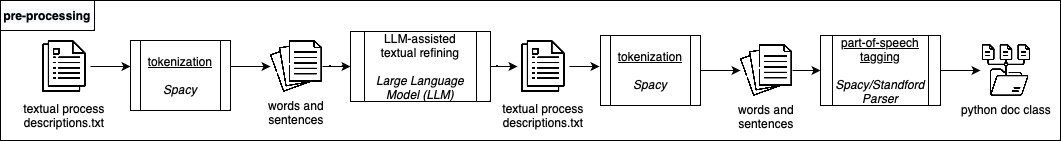
\includegraphics[width=\textwidth]{is-bpm-thesis-latex/vh-resources/preprocessing.png}
\caption{Schematic Overview of the textual data pre-processing workflow. This diagram illustrates the sequence of operations applied to textual process descriptions.} \label{fig1}
\end{figure}

After the LLM-Assisted Textual Refinement (LLM-ATR), the white space and line breaks will be cleaned within the text and the text is broken up into individual words or tokens. Next, the tokens are annotated with part-of-speech (POS) and dependency tags. To finalize the suitable format for the analysis, the data is converted into a standardized format (.doc Python class). 


Modal Identifiers







\subsection{Processing} Processing refers to the stage where the actual analysis takes place. This is the most challenging part due to the complexity of natural language \cite{friedrichProcessModelGeneration2011}. Therefore, a few steps must be performed before refactoring the state-of-the-art approach. 
First, a grammatical label will be assigned to each word in the sentence, indicating whether it is a noun, verb, adjective, adverb, or other part of speech. This task is called part-of-speech (POS) tagging. Second, a Parser is used to analyze the syntactic structure of the sentence and to create a dependency parse tree, which shows how the different tokens are related to each other. Friedrich et al. uses the Stanford Parser, developed by the research laboratory of the University of Sanford. As this approach aims to use the current state of technology, and the last released version of the Stanford Parser (4.2.0) was in 2020 \cite{stanford-nlp}, this approach solves uses the Spacy parser. Third, a Named Entity Recognizer (NER) identifies entities such as people, organizations, and locations in the text and labels them with corresponding entity types.
As our approach follows the current state-of-the-art approach, it continues with the analysis on a sentence level, followed by an analysis on the textual level, the text needs to be spitted into sentences and subsentence. This step is also called boundary detection. For the detection of linguistic boundaries, grammatical labels are used. These grammatic have been created when sentences are spliced into words (tokenization). The detection of boundaries is complicated regarding unexpected grammatical structures or punctuation. 
The example sentence “M.Sc. students are required to apply until tomorrow.” is with standard tools broken into the two following sentences “M.Sc.” and “students are required to apply until tomorrow.”. Therefore, a Matcher can be used to improve the result of boundary detection. The Matcher is a tool for finding sequences of tokens in a text-based on user-defined patterns. These patterns can identify and extract specific entities or relationships between entities in the text. In our case, we use the Matcher to identify specific tokens that indicate a boundary between sentences.
Additionally, the process model does not need example sentences, as BPMN 2.0 diagrams must be atomic \cite{leopoldGeneratingNaturalLanguage2012}. Therefore, example sentences need to be filtered. This can be done by searching in the text for example indicators, such as: for instance, for example, e.g., and removing those (sub)sentences.
Finally, we can start extracting relevant information from the text, starting with the actions. The difficulty here is to decide which information is relevant. Therefore, rules can be defined based on the words’ grammatical labels, which the part-of-speech-tagger has already identified. Next, all objects can be extracted from the sentences and combined with an action based on the grammatical labels. To correctly identify the related action to the object, it is necessary to differentiate between actions in active or passive voice. Due to this, a parameter indicating whether the action is in the active voice or not is set for every identified action. The same steps are repeated to identify actors of the related actions.
As a result of the sentence-level analysis, the extracted actions are stored with the corresponding information in a real-world model. 
\begin{table}[H]
  \begin{center}
    \caption{Lists of indicators for extraction of different BPMN constructions}
    \label{tab:table1}
    \begin{tabular}{l|c|r} % <-- Alignments: 1st column left, 2nd middle and 3rd right, with vertical lines in between
      \textbf{Name of Indicator List} & \textbf{BPMN construction} & \textbf{Examples of Indicators}\\
      \hline
      Condition Indicators & Exclusive gateway & 'if' , 'whether' , 'in case of'\\
      Parallel Indicators & Parallel gateway & 'while', 'meanwhile', 'in parallel'\\
      Sequence Indicators &  For continuation of a branch of a gateway &'then', 'after', 'afterward' \\
      Example Indicators & Example Events & 'for instance', 'for example', 'e.g.' \\
    \end{tabular}
  \end{center}
\end{table}
The previously identified actions still need to include some required information. This is again the case because of the complexity of the natural information: Not all relevant information for an action is stored in one sentence. Therefore, the relations between the sentences are investigated within the text-level analysis part. As an example, anaphors are linguistic methods to avoid repetition. They refer to a word used earlier in a text. To solve this obstacle, anaphor resolution will be used. Next, conditional sentences need to be identified. These sentences use conditional markers, such as “if”, “else” or “otherwise”. As natural language is complicated, it can also consist of multiple words. Or short phrases like “in the meantime” or “in parallel”.
Additionally, these conditional markers have specific characteristics and can be mapped to different BPMN constructions. (See Table). Finally, the information extracted on a text level is added to the information in the world model.

\subsection{Post-processing:} 
After the activities, actors, and relations are determined and extracted in the processing part, post-processing focuses on the visualization of the result. 
Thus, the acquired information will be used to create the four key elements of a BPMN model: events, tasks, gateways, and connecting elements.
To follow the current approach, the first step is to create an initial and complete model. Therefore, nodes are created, sequence flows are built, dummy elements are removed, the open ends are finished, and meta-activities are processed. The initial model is augmented by creating Black Box Pools and Data Objects. Finally, we can layout the model and export it as a .jpg.

\pagebreak

\begin{figure}[H]
    \centering
    \caption{Overview of approach: pre-processing, processing, post-processing}
    \includegraphics[width=0.8\textwidth]{vh-resources/Approach_Overview.jpg}
    \label{fig:Approach_Overview}
\end{figure}
\pagebreak

\section{Categorization of Issues}
\subsection{Relevance of information}
For the generation of the process diagrams, it is important to include only the process relevant information. Additionally, with an increasing number of sentences, the quality of the output decreases \cite{yuImprovedAutogenerationBusiness2023}. Therefore, meta information must be filtered.

A common approach is the use machine learning algorithms to identify irrelevant information. For this approach the algorithm will be trained with using a large dataset.  For this project, this approach is not qualified, as there is a lack of notated process description and regulatory documents. In this approach an LLM is used to filter irrelevant information from the text. To improve the accuracy, few-shot learning is used. Few-shot learning is a machine learning technique that addresses the problem of learning based on a small amount of training data. It enables models to generalize and learn from only a few examples, allowing them to quickly adapt and make accurate predictions with minimal training instances.  This learning approach addresses the limited availability of samples by using meta-learning and regularization techniques.

This classification task is defined as a M-way-K-shot classification. M represents the number of classes and K the number of examples (shots) per class. The performance of this classification tasks depends on the number of classes (M) and the number of shots (K) \cite{parnamiLearningFewExamples2022}.  As the classification task is in this case binary, (0 = irrelevant, 1 = relevant), the number of classes is 2.  The number of examples is depended on the complexity of the classification task. The number of examples per class (K) should be large enough to capture the variability within each class, but not too large to cause over fitting or under fitting. The optimal number of examples per class depends on the specific task and the available data.

//TODO: write ab Example of irrelvant information 

\subsection{Extraction of implicit information}
Implicit information extraction with NLP refers to the process of identifying and extracting information that is not explicitly stated in text but can be inferred from the context. Implicit information is often use to provide descriptive information \cite{pereraKnowledgeDrivenImplicitInformation}.

"The Room Service Manager then submits an order ticket to the kitchen to begin preparing the food."

In this sentence, an explicit action of the room service manager is addressed, but it also implies the action of "preparing food" for the kitchen. 

This issue is especially common in regulatory documents.

„Documented information shall be available as evidence of the implementation of the audit programme(s) and the audit results.“

This sentence implies the relevant process action to „document the results“.

For the generation of complete process diagrams, it is necessary to address this issue and to identify and extract implicit information from text.

To address this issue, the understanding of the content is important. In this work, the implicit information will be detected using LLMs. LLMs are capable of detecting these implicit information and to return it as an explicit information.

Example output for Example XY: //TODO
"The Room Service Manager  submits an order ticket to the kitchen. The kitchen prepares the food.“

Based on these information, NLP will be used to extract the information from the text.

\subsection{Identification of Introduction Sentences}


\subsection{Identification of Actors}
A common approach for the identification of the actors in a text is to use the result of the Named Entity Recognizer and to filter the results based on the results.  


Table XY shows the number of entity tokens (ENTs) recognized by the Spacy standard named entity recognition (NER) for the first four texts of the established gold standard. This is compared to the number of ENTs detected by the PET system. The analysis is limited to these specific texts as they represent the convergent set between our gold standard and the existing PET dataset.

% Move it to evaluation and eplain that it can be replaced
\begin{table}[h]
\centering
\caption{Named Entity Recognition Results}
\label{table:ner_results}
\begin{tabular}{l|l|l}
\textbf{Text} & \textbf{Identified Actor ENTs by Spacy NER} & \textbf{Identified Actor ENTs by PET} \\ \hline
Text 1: & 0 & 8 \\
Text 2: & 0 & 3 \\
Text 3: & 2 & 16 \\
Text 4: & 2 & 8 \\ \hline
\textbf{Total} & \textbf{4} & \textbf{35}
\end{tabular}
\end{table}

%TODO: Maybe in to outlok / discussion 
The spacy default NER can be replaced with an customized model or the default model can be trained by using an annotation tool, such as Prodigy. 

In this approach, we leverage the dependency labels of tokens for the  identification of the actors. Specifically, for active voice sentences, the nominal subject dependency label, \(token.dep_ == "nsubj"\), is utilized. For passive constructions, the agent dependency, denoted as "agent", is considered. Through this approach, the baseline method yields precise outcomes. Given the multifaceted nature of natural language an entity might be referenced using multiple terminologies.

As illustrated in Figure [TODO: Reference to Picture of Text 01 by Shuawei], several actors have been accurately identified. Due to linguistic complexities, two distinct terms reference a singular actor in the example:
\begin{itemize}
    \item Member of the sales department
    \item Sales department
\end{itemize}

In the field of process diagrams, a department is always represented by a representative member. Consequently, the two expressions above refer to a single unit: the sales department.

\textbf{Implementation: } To address the challenge of synonymous terms representing the same actor (as elucidated in Chapter 03), we devised an algorithm. This procedure assesses the similarity between actors prior to appending a new entity to the list of valid actors. This list is subsequently employed for generating both the syntactical structure for the process diagram and the diagram itself.

\begin{algorithm}
\caption{Determine Actor Similarity Utilizing SpaCy's Functionality}
\begin{algorithmic}[1]
\REQUIRE $Actor1: \text{string},  Actor2: \text{string}, nlp:  \text{any}$
\ENSURE $similarity\_score: \text{float}$
\FUNCTION{compare\_actors\_with\_similarity}{$Actor1, Actor2, nlp$}
    \STATE $doc1 \gets nlp(Actor1)$
    \STATE $doc2 \gets nlp(Actor2)$
    \STATE $similarity\_score \gets \text{ROUND}(doc1.\text{similarity}(doc2), 2)$
    \RETURN $similarity\_score$
\ENDFUNCTION
\end{algorithmic}
\end{algorithm}

Algorithm 1 necessitates two actor strings as inputs. For the calculation of similarity we use the inherent functions of SpaCy. Therefore the use of the \("en\_core\_web\_lg"\) pipeline is required and disqualifies the use of the previously used pipeline \("en\_core\_web\_trf"\). This is primarily due to the lack of pre-trained word vectors in the transformer pipeline, which are essential for the similarity estimation process. Each vocabulary term possesses a linked vector, a multi-dimensional construct encapsulating semantic nuances determined by contextual associations in extensive corpora. Derived from the input strings, two SpaCy document objects (Doc) are instantiated. Subsequently, SpaCy's in-built `similarity()` function evaluates the semantic proximity of these documents, contingent on their respective vectors. This operation computes the cosine similarity, interpreting the cosine of the angle delineating two vectors. Cosine similarity values oscillate between -1 and 1. Notably, SpaCy normalizes this value, ensuring the resultant similarity scores range between 0 (indicative of orthogonal vectors, implying dissimilarity) and 1 (identical vectors).

\begin{table}[h!]
\begin{center}
\caption{\centering Similarity between Actors}
\label{table:table1}
\begin{tabular}{c|c|c|c}
    & member of sales department & sales department & member of legal department\\ \hline
member of sales department 		  	&   1      &    0.67    &   0.92 \\
sales department	 				&   0.67   &    1       &   0.46  \\
member of legal department 			&   0.92   &    0.46    &   1 \\ \hline
\end{tabular}
\end{center}
\end{table}

As the cosine similarity, is for "member of legal sales" and "member of legal department" pretty close, but as they refer to different entities, we implemented additionally approach that is token based (TODO: Alg 2). This function is designed to compute a similarity ratio between two actor names by comparing the lemmas (base forms) of their tokens, with an emphasis on significant content words.

Again, given two strings representing actors as input parameters, the function processes them through a predefined natural language processing pipeline, denoted as "nlp", to generate respective Doc objects. Prior to any comparison, the function systematically excludes tokens that are characterized as "stop words". Stop words, refer in linguistics and natural language processing to frequently occurring words in a language that, in analytical contexts, are considered to offer limited semantic value. Subsequently, the function undertakes a pairwise comparison of the lemmas of the tokens derived from the two actors. The objective of this phase is to enumerate the quantity of matching lemmas between the two sets. Acknowledging the potential variance in token counts between different actor strings, the function uses a normalization procedure to ensure a balanced evaluation of similarity without distortion.

\begin{algorithm}
    \caption{Compare Actor Tokens Using SpaCy}
    \label{}
    \begin{algorithmic}[1]
        \REQUIRE $Actor1: \text{string},  Actor2: \text{string}, nlp: \text{any}$
        \ENSURE $similarity\_ratio: \text{float}$
        %\FUNCTION{compare\_actors\_with\_token}{$Actor1, Actor2, nlp$}
            \STATE $doc1 \gets nlp(Actor1)$
            \STATE $doc2 \gets nlp(Actor2)$
            \STATE $tokens1 \gets \text{FILTER\_OUT\_STOP\_WORDS}(doc1)$
            \STATE $tokens2 \gets \text{FILTER\_OUT\_STOP\_WORDS}(doc2)$
            \STATE $num\_tokens1 \gets \text{length}(tokens1)$
            \STATE $num\_tokens2 \gets \text{length}(tokens2)$
            \STATE $matching\_tokens \gets 0$
            \IF{$num\_tokens1 \leq num\_tokens2$}
                \FOR{each $token1$ in $tokens1$}
                    \FOR{each $token2$ in $tokens2$}
                        \IF{$token1.lemma\_ == token2.lemma\_$}
                            \STATE $matching\_tokens \gets matching\_tokens + 1$
                            \STATE \textbf{break}
                        \ENDIF
                    \ENDFOR
                \ENDFOR
            \ELSE
                \FOR{each $token2$ in $tokens2$}
                    \FOR{each $token1$ in $tokens1$}
                        \IF{$token2.lemma\_ == token1.lemma\_$}
                            \STATE $matching\_tokens \gets matching\_tokens + 1$
                            \STATE \textbf{break}
                        \ENDIF
                    \ENDFOR
                \ENDFOR
            \ENDIF
            \STATE $avg\_tokens \gets (num\_tokens1 + num\_tokens2) / 2.0$
            \IF{$avg\_tokens > 0$}
                \STATE $similarity\_ratio \gets matching\_tokens / avg\_tokens$
            \ELSE
                \STATE $similarity\_ratio \gets 0.0$
            \ENDIF
            \RETURN $similarity\_ratio$
        %\ENDFUNCTION
    \end{algorithmic}
\end{algorithm}

member of legal department
member of sales department
sales department

\subsection{Custom Sentencizer wit LS}
\subsection{Including Sentences}
\section{}
\subsection{}
\subsection{More Actors}

NLP is for unstructured texts






not easily translated into other languages when ISO documents are used around the world. 
ISO defines the following 
"may” to express a permission  
“can” to express a possibility or capability
The words “might” or “could” should not be used to avoid confusion and misapplication of the text


Numbering

10 Test report

10.1 Requirements

The test report shall include the following information:

a) the sample
b) a reference to this document, i.e. ISO 1234:2020;
c) the method used;
d) the result;
e) any deviations from the procedure;
f) any unusual features observed;
g) the date of the test.

10.2 Optional
It may also include:

a) the test schedule;
b) the test operator.


\begin{algorithm}
    \caption{Preprocess Textual Description with LLM}
    \label{}
    \begin{algorithmic}[1]
        \REQUIRE $text\_input: \text{string}$
        \ENSURE $response: \text{string}$
            \STATE $prompts \gets [] $
            \STATE $add prompts to prompts$
            \STATE $history \gets []$
            \STATE $response = text\_input$
            \FOR{each $prompt$ in $prompts$}
                \STATE $response, history \gets chatbot(prompt + response, history)$
            \ENDFOR 
        \RETURN $response$
    \end{algorithmic}
\end{algorithm}

\begin{algorithm}
    \caption{Chatbot}
    \label{}
    \begin{algorithmic}[1]
        \REQUIRE $input: \text{string}, history: \text{None \OR dict}$
        \ENSURE $response: \text{string}$
            \STATE $prompts \gets [] $
            \STATE $add prompts to prompts$
            \STATE $history \gets []$
            \STATE $response = text\_input$
            \FOR{each $prompt$ in $prompts$}
                \STATE $response, history \gets chatbot(prompt + response, history)$
            \ENDFOR 
        \RETURN $response$
    \end{algorithmic}
\end{algorithm}

Mit dem pre processing der Texte wollten wir folgende Kriterien sicherstellen:
1. 
2.
3.

Die Herausforderung hierbei war das prompt engineering. Therefore we tried multiple approaches:
1. Defining all criteria in one prompt 
2. Defining all criteria in one prompt + adding examples (shots)
3. Splitting the criteria into multiple prompts with their examples and using the response from the last result for the next prompt as text. First prompt was with intital text description 
4. Using a chat construct to build an history

intro = """You are a system analyst, that strictly and carefully follows the instructions. 
        You return the output text in full sentences without adding any extra information, interpretation, explanation, numberations or listings. 
        Make sure that the previously given instructions are still followed.
        You handle every task sentence for sentence. \n"""


Auswahl eines trainierten LLMs.

Each Prompt is structured like this:

### Instruction: #### \n
     
## Examples: ## . \n
            
###### TEXT ###### \n


The organization shall identify what needs to be monitored and measured. The organization shall select the methods for monitoring, measurement, analysis and evaluation. The organization shall specify when the monitoring and measuring shall be performed. The organization shall designate who shall monitor and measure. The organization shall determine when the results from monitoring and measurement shall be analysed and evaluated. The organization shall assign who shall analyse and evaluate these results. The organization shall document the results as evidence. The organization shall assess the information security performance and the effectiveness of the information security management system.


For the extraction of information from regulatory some requirements are necessary to be fulffilled before the text is processed with rule-based NLP techniques:



